% Author: Izaak Neutelings (November 2020)
\documentclass[border=3pt,tikz]{standalone}
\usepackage{amsmath} % for \text
\usepackage{tikz}
\tikzset{>=latex} % for LaTeX arrow head
%\usetikzlibrary{patterns} % for hatches area

% colors
\colorlet{mylightred}{red!50!black!15}
\colorlet{mylightblue}{blue!50!black!15}
\colorlet{mylightgreen}{green!50!black!15}


\begin{document}


% CONTROL REGIONS FF
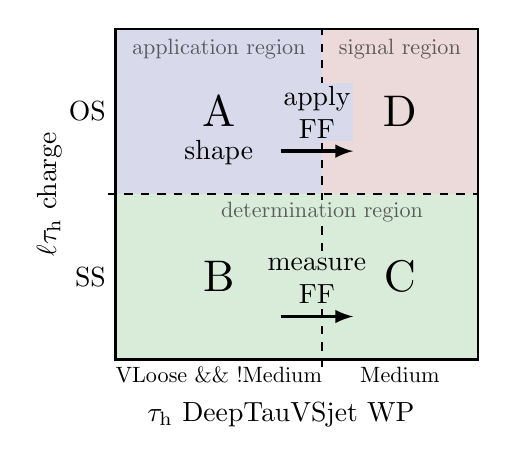
\begin{tikzpicture}
  \def\xmax{4.6}
  \def\ymax{4.2}
  \def\mx{0.57*\xmax}
  \def\my{0.50*\ymax}
  
  % boxes
  \fill[mylightblue] (0,\my) rectangle (\mx,\ymax); % A
  \fill[mylightgreen](0,0) rectangle (\xmax,\my); % SS = B + C
  \fill[mylightred] (\mx,\my) rectangle (\xmax,\ymax); % D
  \draw[thick] (0,0) rectangle (\xmax,\ymax);
  
  % dashed lines
  \draw[dashed,thick] (\mx,-0.1) -- (\mx,\ymax);
  \draw[dashed,thick] (-0.1,\my) -- (\xmax,\my);
  
  % labels
  \draw
    (0,{\ymax+\my)/2}) node[left]  {OS}
    (0,\my/2) node[left]  {SS}
    (\mx/2,0) node[below,scale=0.8] {VLoose \&\& !Medium}
    ({(\xmax+\mx)/2},0) node[below,scale=0.8] {Medium}
    (0,\my) node[rotate=90,above=16pt] {$\ell\tau_\mathrm{h}$ charge}
    (\my,0) node[below=12pt] {$\tau_\mathrm{h}$ DeepTauVSjet WP};
  \draw
    (\mx/2,{\ymax+\my)/2}) node[scale=1.6] {A}
    (\mx/2,{\my+0.25*(\ymax-\my)}) node[scale=1.0] {shape}
    (\mx/2,\my/2) node[align=center,scale=1.6] {B}
    ({(\xmax+\mx)/2},\my/2) node[align=center,scale=1.6] {C}
    ({(\xmax+\mx)/2},{\ymax+\my)/2}) node[scale=1.6] {D};
  \draw[->,very thick]
    (0.8*\mx,0.26*\my) --++ (0.2*\xmax,0)
    node[midway,above=3,align=center,fill=mylightgreen,inner sep=1] {measure\\FF};
  \draw[->,very thick]
    (0.8*\mx,{\my+0.26*(\ymax-\my)}) --++ (0.2*\xmax,0)
    node[midway,above=3,align=center,fill=mylightblue,inner sep=1] {apply\\FF};
  \node[below=2,scale=0.8,mylightgreen!40!black,fill=mylightgreen,inner sep=1] at (\mx,\my) {determination region};
  \node[below=1,scale=0.8,mylightblue!40!black] at (\mx/2,\ymax) {application region};
  \node[below=1,scale=0.8,mylightred!40!black] at ({(\xmax+\mx)/2},\ymax) {signal region};
  
\end{tikzpicture}


% CONTROL REGIONS FF
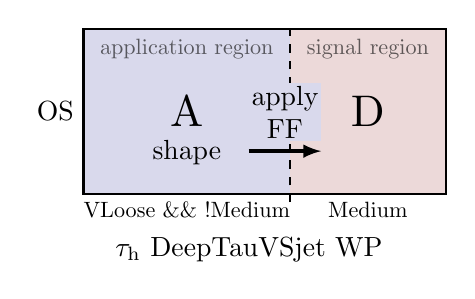
\begin{tikzpicture}
  \def\xmax{4.6}
  \def\ymax{4.2}
  \def\mx{0.57*\xmax}
  \def\my{0.50*\ymax}
  
  % boxes
  \fill[mylightblue] (0,0) rectangle (\mx,\ymax-\my); % A
  \fill[mylightred] (\mx,0) rectangle (\xmax,\ymax-\my); % D
  \draw[thick] (0,0) rectangle (\xmax,\ymax-\my);
  
  % dashed lines
  \draw[dashed,thick] (\mx,-0.1) -- (\mx,\ymax-\my);
  
  % labels
  \draw
    (0,{\ymax-\my)/2}) node[left]  {OS}
    (\mx/2,0) node[below,scale=0.8] {VLoose \&\& !Medium}
    ({(\xmax+\mx)/2},0) node[below,scale=0.8] {Medium}
    (\my,0) node[below=12pt] {$\tau_\mathrm{h}$ DeepTauVSjet WP};
  \draw
    (\mx/2,{\ymax-\my)/2}) node[scale=1.6] {A}
    (\mx/2,{0.25*(\ymax-\my)}) node[scale=1.0] {shape}
    ({(\xmax+\mx)/2},{\ymax-\my)/2}) node[scale=1.6] {D};
  \draw[->,very thick]
    (0.8*\mx,{0.26*(\ymax-\my)}) --++ (0.2*\xmax,0)
    node[midway,above=3,align=center,fill=mylightblue,inner sep=1] {apply\\FF};
  \node[below=1,scale=0.8,mylightblue!40!black] at (\mx/2,\ymax-\my) {application region};
  \node[below=1,scale=0.8,mylightred!40!black] at ({(\xmax+\mx)/2},\ymax-\my) {signal region};
  
\end{tikzpicture}



\end{document}